% This must be in the first 5 lines to tell arXiv to use pdfLaTeX, which is strongly recommended.
\pdfoutput=1
% In particular, the hyperref package requires pdfLaTeX in order to break URLs across lines.

\documentclass[11pt]{article}

% Remove the "review" option to generate the final version.
\usepackage[]{acl}

% Standard package includes
\usepackage{times}
\usepackage{latexsym}
\usepackage{graphicx}
\graphicspath{ {./images/} }
\usepackage{epigraph}

% For proper rendering and hyphenation of words containing Latin characters (including in bib files)
\usepackage[T1]{fontenc}
% For Vietnamese characters
% \usepackage[T5]{fontenc}
% See https://www.latex-project.org/help/documentation/encguide.pdf for other character sets

% This assumes your files are encoded as UTF8
\usepackage[utf8]{inputenc}

% This is not strictly necessary, and may be commented out,
% but it will improve the layout of the manuscript,
% and will typically save some space.
\usepackage{microtype}

% This is also not strictly necessary, and may be commented out.
% However, it will improve the aesthetics of text in
% the typewriter font.
\usepackage{inconsolata}

% If the title and author information does not fit in the area allocated, uncomment the following
%
%\setlength\titlebox{<dim>}
%
% and set <dim> to something 5cm or larger.

\title{Analizing disfluences in HCI}

% Author information can be set in various styles:
% For several authors from the same institution:
% \author{Author 1 \and ... \and Author n \\
%         Address line \\ ... \\ Address line}
% if the names do not fit well on one line use
%         Author 1 \\ {\bf Author 2} \\ ... \\ {\bf Author n} \\
% For authors from different institutions:
% \author{Author 1 \\ Address line \\  ... \\ Address line
%         \And  ... \And
%         Author n \\ Address line \\ ... \\ Address line}
% To start a seperate ``row'' of authors use \AND, as in
% \author{Author 1 \\ Address line \\  ... \\ Address line
%         \AND
%         Author 2 \\ Address line \\ ... \\ Address line \And
%         Author 3 \\ Address line \\ ... \\ Address line}

\author{Guillem Gili i Bueno\\
	University of Potsdam\\
	\texttt{giliibueno@uni-potsdam.de}}

\begin{document}
	\maketitle
	\begin{abstract}
		In this document we analyze the disfluences that happen when a human interacts with a robot. Specifically we will focus on self-repair disfluences, that happen in utterances that happen within the same turn of a speaker (in this case the human). We also compare the differences in this behavior when interacting with a robot rather than a human. We try and make sense of the differences from rigorous studies and our results hint a bit at the fact that self-repair may also be affected by alignment.
	\end{abstract}

\section{Introduction}

The phenomena of \emph{Disfluences} refers to morphosyntactical irregularities that happen in spoken dialogue including fillers("um","eh")  and corrections to previous words (Figure \ref{fig_disfluence_example}). 
\begin{figure}[h]

\centering
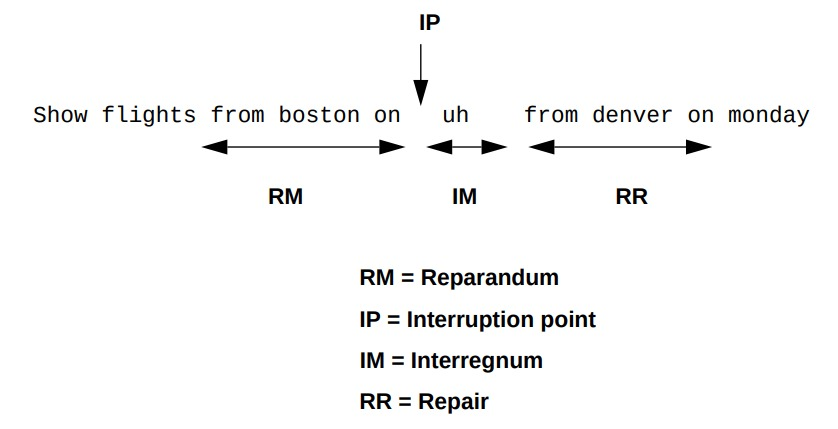
\includegraphics[width=0.45\textwidth]{disfluences_example}
\caption{\emph{Disfluence} example extracted from \cite{shriberg1994preliminaries}, one of the most comprehensive works on \emph{Self-repair} in English}
	\label{fig_disfluence_example}
\end{figure}

When we do \emph{Disfluences}, one of the methods to mitigate confusions is to use \emph{Repair}. In this project I will be alway talking about \emph{Self-repair} as the Self-Initiated \emph{Self-repair}, but it is worth mentioning that it can be Other-Initiated. \emph{Self-repair} refers to the act of stopping within the utterance to correct what the same speaker was in the process of saying. In particular I will focus on the replacement and recycling repair types.


Another phenomena we must cover is \emph{Alignment}. \emph{Alignment} is defined in \cite{pickering_garrod_2004}:
\begin{quote}
[...] interlocutors tend to
develop the same set of referring expressions to refer to
particular objects, and that the expressions become shorter
and more similar on repetition with the same interlocutor
and are modified if the interlocutor changes [...] 
\end{quote}

The support for this definition comes from research in priming (evoking an inadverted change in dialogue) syntactically \cite{Branigan2000} and lexically\cite{bock1986meaning}. And in the same paper where we borrowed the definition for \emph{Alignment}, the following extension is made regarding dialogue specifically:

\begin{quote}
	[...] This occurs by priming mechanisms at each level of linguistic representation, by percolation between the levels so that alignment at one level enhances alignment at other levels, and by repair mechanisms when alignment goes awry. [...]
\end{quote}




\section{Related work}

\subsection{Motivations}

\emph{Self-repair} is well-established and classified in many languages, e.g. English \cite{shriberg1994preliminaries}, Japanese \cite{hayashi1994comparative}, Indonesian \cite{wouk2005syntax}. The studies across these show evidence that \emph{Self-repair} is both inconsistent across different languages and highly conventionalized (e.g. Figure \ref{placeholder_repair_jap},\ref{recycling_eng},\ref{recycling_jap}). Further evidence for these properties can be found easily in other papers \cite{fox20102487}.  
\begin{figure}[h]
	
	\centering
	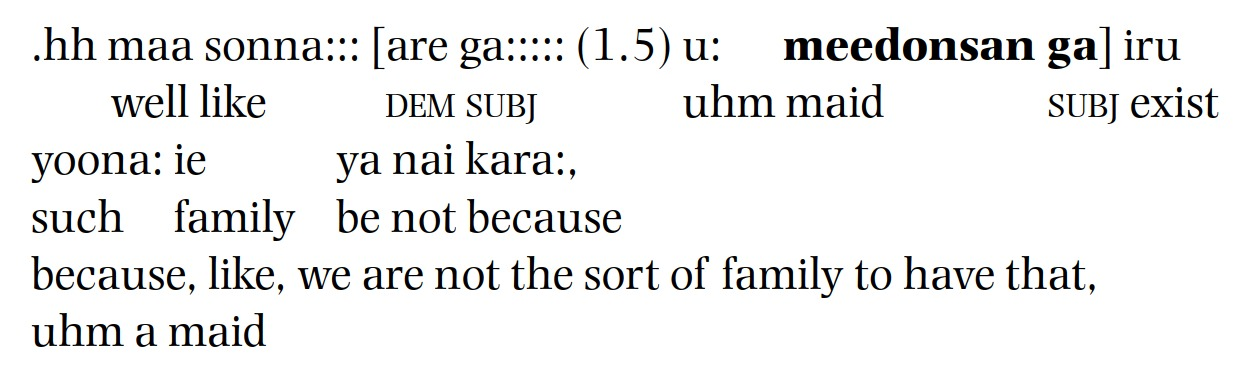
\includegraphics[width=0.45\textwidth]{placeholder_repair_jap}
	\caption{Placeholder repair example extracted from \cite{wouk2005syntax}. This type of \emph{Self-repair} does not exist in English}
	\label{placeholder_repair_jap}
\end{figure}


\begin{figure}[h]
	
	\centering
	
\includegraphics[width=0.45\textwidth]{recycling_eng}
	\caption{\emph{Self-repair} examples extracted from \cite{wouk2005syntax}. \emph{Self-repair} after a Direct Object recycles a whole constituent (rather than only the verb). This does not happen in Japanese.}
	\label{recycling_eng}
\end{figure}


\begin{figure}[h]
	
	\centering
	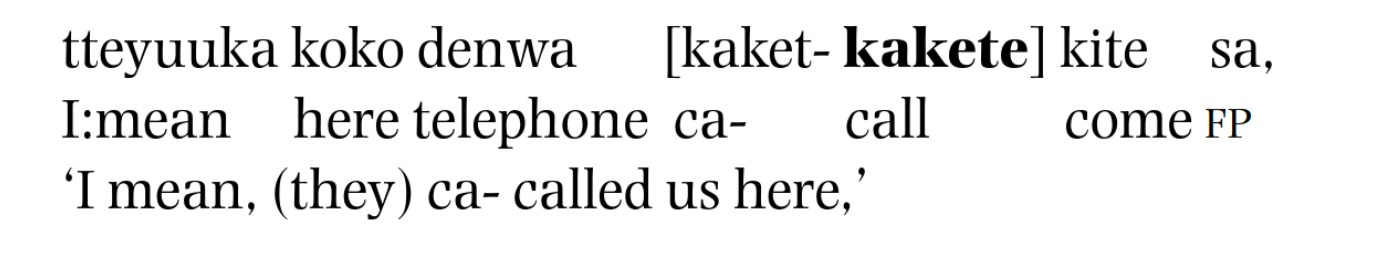
\includegraphics[width=0.45\textwidth]{recycling_jap}
	\caption{\emph{Self-repair} example extracted from \cite{wouk2005syntax}. \emph{Self-repair} in Japanese of the direct constituent (verb), rarer in English.}
	\label{recycling_jap}
\end{figure}



It would seem likely that the two phenomena, \emph{Alignment} and \emph{Self-Repair} (not present in robotic speech), could alter the human dialogue both in the rate  and type of \emph{Self-repair}. On one hand it is likely that a human tries to \emph{Self-repair} less, due to trying to align to said robotic speech. It is also entirely possible that the effect on \emph{Self-repair} is the opposite, since our second quote from \cite{Branigan2000} points that \emph{Self-repair} is precisely used when aligning mechanisms go awry. Regarding the type of \emph{Self-repair}, for example, some substitutions may replace with pronouns less due to a perceived minimal common ground with the robot.


Furthermore, \emph{Alignment} is not limited to the aspects listed in the original paper \cite{pickering_garrod_2004}, \emph{Alignment} happens in several modalities, quoting from \cite{branigan2010linguistic}:

\begin{quote}
	[...] interlocutors tend to align on accent
	and speech rate [...] adopt increasingly similar phonetic realizations of repeated words [...]  repeat each other in terms of their grammatical choices [...] 
\end{quote}



In the same paper \cite{branigan2010linguistic}, several other motivations for \emph{Alignment} (passive) adaptations are mentioned that may be relevant in HCI:
\begin{quote}
	[...] cognitive economy that they offer, since they do not require the speaker to model her interlocutor [...]  might also serve a different strategic purpose, related to the social relationships between the participants in the interaction [...] 
\end{quote}

It is possible that one may not find the motivations listed when interacting with a robot. On another hand, the paper does also compile a lot of evidence on alignment happening when a person interacting in a Wizard of Oz paradigm believed the other agent to be a robot (less pronoun usage, happened in the reverse Wizard of Oz paradigm as well). Other syntax and lexical alignment is mentioned to happen, even to a higher degree in HCI \cite{branigan2003syntactic}.



\subsection{Data}

Data availability is limited when researching dialogue datasets online. Not only that, manual analysis for this data is challenging: costly in time and effort, requires education prior to being done and revision is very advisable. 

My first intention on this study was to look at data from other existing publications and try to draw a quantitative comparison on the data obtained from our HCI samples to those. Given the limited amount of samples in experimentation I don't think it is valid drawing the comparison another original paper; regardless I will go over it for these reasons:
\begin{itemize}
	\item The initial study proposal (HCI and its effects on self-repair quantitatively) is valid and interesting.
	\item If in the future someone decides to do this study (myself included) with larger amounts of data and more rigorous conditions, I would hope to lighten their work on research.
	\item Some of the observations on the data papers may be applicable to the data I obtain or explain some behavior.
\end{itemize}


The data I intended to use is in Replacement and Recycling in English  according to syntactic category  \cite{fox20102487} and can be seen in Figure \ref{fox_replacement}. In this case the most common recycle destination (where we jump back for recycling) by a large margin are subject pronouns, followed by determiners, wh-words and prepositions. On the other hand the replaced item has a more even distribution (except wh-words, auxiliars and existentials) but Nouns are appear to be much more commonly replaced. We can also see that Function words predominate as recycle destination and replaced item, where as content words are rarer. It would be expectable to see at least see the most common substitutions happen often in our study.

\begin{figure*}[h]
	
	\centering
	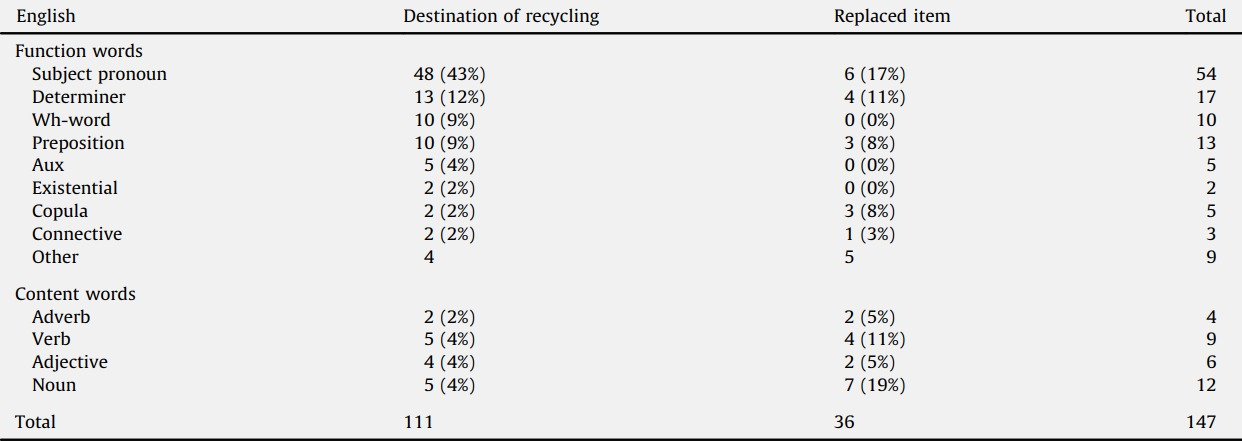
\includegraphics[width=\textwidth]{fox_replacement}
	\caption{\emph{Self-Repair} substitutions by type \cite{fox20102487}}
	\label{fox_replacement}
\end{figure*}






\section{Task Formalisation}

\subsection{Context}

The objective is to study the occurrance of Self-Repair. This was a deliberate choice, since Disfluences are relatively common in dialogues and the amount of data available and time to dedicate is limited. In the design, we noticed the following requirements:
\begin{itemize}
	\item \textbf{Naturality} We want the dialogue to ressemble an average human-to-human conversation; since the HCI is already rigid enough we want to at least minimize the amount of issues that could happen in the conversation
	\item \textbf{Bi-lateral communication} It is important that both the human and robot interact in meaningful ways, as to elicit the alignment properly if it were to happen. One-sided conversations will not work for us.
\end{itemize}

Given those constraints, we decided on \textbf{a role-play situation where the human would get interview advice from a robot}. This has several advantages:
\begin{itemize}
	\item The speaker has a goal unrelated to the phenomena we want to study which should help with naturality.
	\item Role-playing parenthesis happen naturally, which help with clarification requests (another team member required them).
	\item Balanced turns should happen more or less naturally.
\end{itemize}

It is worth noting that we initially considered using an LLM combined with some incremental model \cite{schlangen2011general} for simplicity of development and naturality. However, this option was discarded as the overhead from including new functionalities would have added much more work, and it was decided to do a more hardcoded implementation. We still think that this would be an interesting idea, but beyond the scope for this project.

\subsection{Implementation}

We used the Furhat environment for implementing our robot agent, as is required per the subject. The interaction was designed always allowing to request dialogue options to the robot, and upon selection of an option the robot asked an open question (to elicit a bit of conversation from the participant) and then gave a bit of trivia (2-3 sentences). There were 2 broad fields (Resumé and Job Interview) and each field had 3 interactions where slots could be filled. Upon successfully requesting one of the interactions there was a 1/5th chance of the robot doing a clarification request. The agent also reminded after every slot filling which slots on the broad field were filled, to remind the user of what had been said. The full interaction diagram can be seen in Figure \ref{flow_diagram}.


\begin{figure}[h]
	
	\centering
	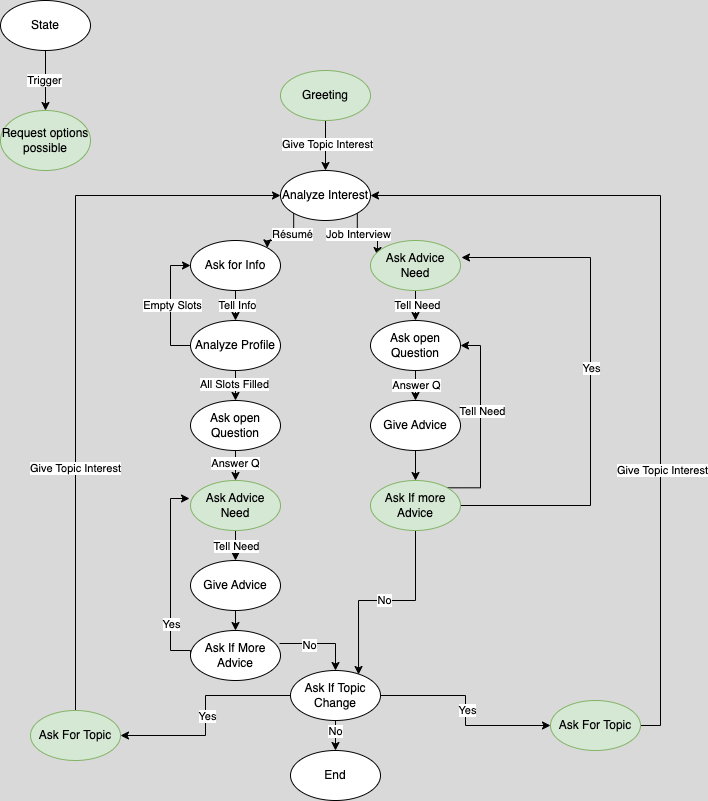
\includegraphics[width=0.45\textwidth]{flow_diagram}
	\caption{Flow diagram for our agent}
	\label{flow_diagram}
\end{figure}

While the interaction with the robot itself was less natural than we would have wanted it do, for the purpose of eliciting natural Self-Repair this implementation proved to be enough. We would have preffered more naturality in the conversation to distract the human from our research, but from listening to the audios the goal the participants chose was  to explore the dialogue options. This proved to be an equally valid distraction.


\section{Experiments}

At the beginning of the experiment the participants were told the general context for their conversation with the robot (the robot giving interview advice) and that they could request their options at any time. Figure \ref{set_up} shows the setup. We reduced the interaction for Furhat to 2 meters, which in the experiment room ensured nobody else was captured by it. The human interacting with furhat was facing the windows (on a 2nd floor and blocked inmediately by another building) to try and minimize the distractions that could affect him/her. All our project members were present during the recording, we tried interacting minimally with the speaker and only intervene in some specific instances where the speaker was using an unrecognizable words by the language detection algorithm ("Say cv instead of resume"). Our assistants' voice was never captured by Furhat, and we only addressed the participant. Transcriptions only include the proper Furhat interaction, not necessarily the introduction to the task even though that is in the audio. We encouraged participants on open questions to talk a bit further on open questions.


A consent form was given prior to the interaction and an evaluation form given at the end, these can be found within the project in the "forms" folder \cite{xarxaxdev-FurhatInterviewRobot} \footnote{This repo is private, request can be granted asking me or another contributor.}. The data from the experiment is also accessible in the repo at the moment of writing this report, but we cannot make it public as is stated in the consent form.

\begin{figure}[h]
	
	\centering
	
\includegraphics[width=0.45\textwidth]{set_up}
	\caption{Set up for the interaction}
	\label{set_up}
\end{figure}

Only audio was collected for the purpose of our research since no team member decided to work on gestures. This was collected from a computer right near Furhat to ensure audio was received intensely enough and slight testing was done prior to it.


\section{Data Analysis}

I have excluded the data from 2 participants due to not meeting minimum validity criteria. During Participant \#1's conversation, some technical issues happened with the code and the dialogue looped, making the overall conversation quite jarring and long without really much interaction and a lot of repetition. After that the code issues were fixed. Participant \#6 was extremely confused during all the interaction; which resulted in an extremely disconnect dialogue and has been excluded as well. This leaves us with a total of 5 dialogues and slightly below 30 minutes of recording. 

There are only a total of 9 Self-Repair examples. Minimal context has been kept to show from where the disfluence originates. Participants 2,3,4,5 and 7 made respectively 2,1,0,5 and 1 Self-Repairs. These can be read in the Appendix \ref{sec:appendix}.

Figures \ref{selfrepair_13} and \ref{selfrepair_25} show an articulation error, which are usually quite rare. I would assume the increased pressure from a limited window to respond to the robot (after some tries where the robot interrupted the user) are the cause for these.

Regarding the destinations of recycling: Figures \ref{selfrepair_12},\ref{selfrepair_15},\ref{selfrepair_35},\ref{selfrepair_45},\ref{selfrepair_55}, all show examples where the destination is a wh-word, Figures \ref{selfrepair_35},\ref{selfrepair_17} show a pronoun and Figure \ref{selfrepair_22} shows a preposition. If we look back at the statistical data we have \cite{fox20102487} we can that these are 3 of the top 4 categories and we have no other examples that use another recycling point. While we would be expecting the Pronoun to be the most prevalent category, the setup for the interaction (requesting options being is very prevalent tool for the human interacting with the robot) probably explains the wh-words being much more common. In Figure \ref{selfrepair_12} it is worth noting that in the first of two consecutives repairs the repair destination happens on a verb; but it is a modal verb with a role equivalent to an wh-word.


Regarding the replaced item, we really only have examples on Figures \ref{selfrepair_12} (Modal verb,Wh-word), \ref{selfrepair_35} (Verb) and \ref{selfrepair_17} (Subject Pronoun). The data once again matches our reference paper \cite{fox20102487}, but differs in the prominence of Wh-words. I once again interpret this as a results of the setting of the conversation.

In my opinion, the unusual prevalence of wh-words unlike in our literature \cite{fox20102487} is due to the combination of two general factors (besides the setup). First, in  English self-repair tends to have as a destination word the beginning of a syntactic structure rather than the last word; when this happens it is out of convenience rather than convention. Second, I would imagine in HCI (or at the very least in interactions with Furhat) full-utterance repairs are much more prevalent. Quite often the robot will not be listening or will focus only in the sentence that it can recognize. Noticing this, participants may have a much higher preference for recycling the sentence alltogether. This could be seen as an alignment in the sense that participants may be trying to match the "only full utterances" of our robot and suggests that alignment also happens in conventionalized situations in general.

\section{Conclusion}

We have seen some evidence that the setup is extremely relevant to the types of repairs we can expect in an interaction. We also have some data that suggests that alignment does happen even in robotic speech; even when the motivating factors behind it do not happen. The fact rigorous evidence \cite{fox20102487} points to alignment happening across HCI and that combined with the results of this study suggest the conventionalized Self-Repair mechanics to be another aspect of alignment. Further research needs to be done in this aspect to confirm this point.

\section{Limitations and Ethical Considerations}

During data collection, a lot of irregularities or bad practices happened that I will go over. This does not make the research on other papers and the observations put together less valid, but the data obtained on our team's experiments should be taken with a grain of salt. As much as I have tried to be rigorous in its analysis, there are factors that make the data obtained not rigorous enough for an official research:
\begin{itemize}
	\item All the participans (2 through 7) were familiar with the robot technology, knew how to develop an interaction itself. A conversation where you are aware of the limitations is heavily biased.
	\item The amount of participants and data is extremely low. While I have related the instances of self-repair to our data, the samples are just too few to have any statistical significance. 
	\item Some participants had some exposure to the experiment prior to participating. This was inevitable, as the room we were using for experimentation linked the other group's experiment and the outside.
	\item Our team encouraging on talking more when responding to open questions makes the data less rigorous as well.	
	\item While we did our best implementing the interaction, the final result was quite jarring to work with. Repeating multiple times the same sentences, being interrupted in unusual situations and navigating the interaction with the robot itself. Those 3 factors for sure fatigued or annoyed the participants, and that may bias the results. It also probably the shifted the conversation from a dialog to maze-solving, or something akin to talking to an interactive book.
	In hindsight this may be a better idea for the setting of an experiment, as this also puts a goal unrelated to phenomena to study and may be more fun for the participant.
\end{itemize}

% Entries for the entire Anthology, followed by custom entries
\bibliographystyle{APA}
\bibliography{custom}

\appendix
\clearpage
\section{Appendix}
\label{sec:appendix}

\begin{figure}[!h]
\begin{quote}
R: Interesting. What kind of advice about writing a cv were you looking for?\\
H: How to write\\
R: I didn't get that, sorry. Try again.\\
H: How to write\\
R: I still didn't get that, sorry. Could you rephrase?\\
H: Hm... Can I ask my - How are - What are my options\\
\caption{Self-Repair Example 1 on Participant 2}
\label{selfrepair_12}
\end{quote}
\end{figure}


\begin{figure}[!h]
\begin{quote}
H: I would like to know how to , uh , <overlap> write the content <overlap>\\
R: <overlap> Still couldn't <overlap> get that. Let's start over. What kind of advice about writing a cv were you looking for? \\
H: I wanna know about - about the content of my resume.
\caption{Self-Repair Example 2 on Participant 2}
\label{selfrepair_22}
\end{quote}
\end{figure}


\begin{figure}[!h]
\begin{quote}
R: I see. How do you personally prepare for an interview?\\
H: Um, I guess I would look up the company details, aand, uh, try to anpici-anticipate the questions.
\caption{Self-Repair Example 1 on Participant 3}
\label{selfrepair_13}
\end{quote}
\end{figure}


\begin{figure}[!h]
\begin{quote}
	H: Well with what can you help me with?\\
	R: I didn't get that, sorry. Try again.\\
	H: What uh, what are my options what eh what-what do you - what can you help me with?  
\caption{Self-Repair Example 1 on Participant 5}
\label{selfrepair_15}
\end{quote}
\end{figure}

\begin{figure}[!h]
\begin{quote}
R: How many years of experience do you have in your field?\\
H: em, workwise eh I got my first job in 2018 so this is 5 years now alm-almost yeah
	\caption{Self-Repair Example 2 on Participant 5}
	\label{selfrepair_25}
\end{quote}
\end{figure}

\begin{figure}[!h]
\begin{quote}
	R: So you have a master's degree, have worked in 2 roles and have 5 years of working experience. What are your concerns when it comes to writing a CV?\\
	H: No, I've- I have a bachelor's degree, you misunderstood me ah, sorry. 
	
	\caption{Self-Repair Example 3 on Participant 5}
	\label{selfrepair_35}
\end{quote}
\end{figure}

\begin{figure}[!h]
\begin{quote}
	H: Um, I don't know. I mean, what advice can you offer?\\
	R: I didn't get that sorry. Try again. \\
	H: Em, what-what-what tips do you have for writing a cv? What are my options?
	\caption{Self-Repair Example 4 on Participant 5}
	\label{selfrepair_45}
\end{quote}
\end{figure}

\begin{figure}[!h]
\begin{quote}
	R: I still didn't get that, sorry. Could you rephrase? \\
	H: What are - what are my options?
	\caption{Self-Repair Example 5 on Participant 5}
	\label{selfrepair_55}
\end{quote}
\end{figure}

\begin{figure}[!h]
\begin{quote}
	R: So you have a Bachelor Degree, have worked in 1 roles and have 3 years of working experience. What are your concerns when it comes to writing a CV?\\
	H: I don't know what the companies want to see on the cv, I don't know which one I should - which of my abilities, which of my education and what is the most important thing that I should display in it.
	\caption{Self-Repair Example 1 on Participant 7}
	\label{selfrepair_17}
\end{quote}
\end{figure}

\end{document}
